\begin{usecase}{Suggest Conflict Resolutions}
  \ucbasicinfo{High}{Regular}
  \ucshortdescription{This UC gives the user all the conflicts and possible ways to resolve it.}
  \uctrigger{The UC is triggered when a conflict is detected between any overlapping event}
  \ucactors{User}{WhatsApp}
  \ucpreconditions{The calendar must have events}
  \ucrelationships{N/A}{Manage Scheduling Conflicts}{N/A}
  \ucinputsoutputs{
    \begin{itemize}
      \item \textbf{Overlapping events} (Source: Saved Events in Database)
      \item \textbf{User suggested resolution} (Source: User)
    \end{itemize}
  }{
    \begin{itemize}
      \item \textbf{Resolution options} (Destination: User Interface)
      \item \textbf{Updated calendar schedule} (Destination: Calendar)
    \end{itemize}
  }
  \ucmainflow{
    \begin{enumerate}
      \item The system detection conflicts
            \ucinfo{The system detects overlapping of events either added manually or extracted from WhatsApp and gives a notification to the user.}
      \item The system gives the suggestions for Conflicts.
            \ucinfo{The system provides the user with the list of resolution options.
              \begin{itemize}
                \item By moving the overlapping event to another time slot.
                \item Keep both events with a conflict warning.
              \end{itemize}}
    \end{enumerate}
  }
  \ucalternateflows{
    \begin{enumerate}
      \item {No conflicts detected}
    \end{enumerate}
  }
  \ucexceptions{
    \begin{itemize}
      \item If the system doesn't get any possible way to resolve the conflict then the system would mark both the event as conflicting.
    \end{itemize}
  }
  \ucconclusion{The UC ends when the user chooses resolution weather if to reschedule the event or leaving it without resolving and it is reflected in on the calendar.}
  \ucpostconditions{The conflicting events in the calendar are either resolved or marked as conflicting}
  \ucspecialrequirements{The system give feasible conflict resolution options}
\end{usecase}

\begin{figure}[!h]
  \centering
  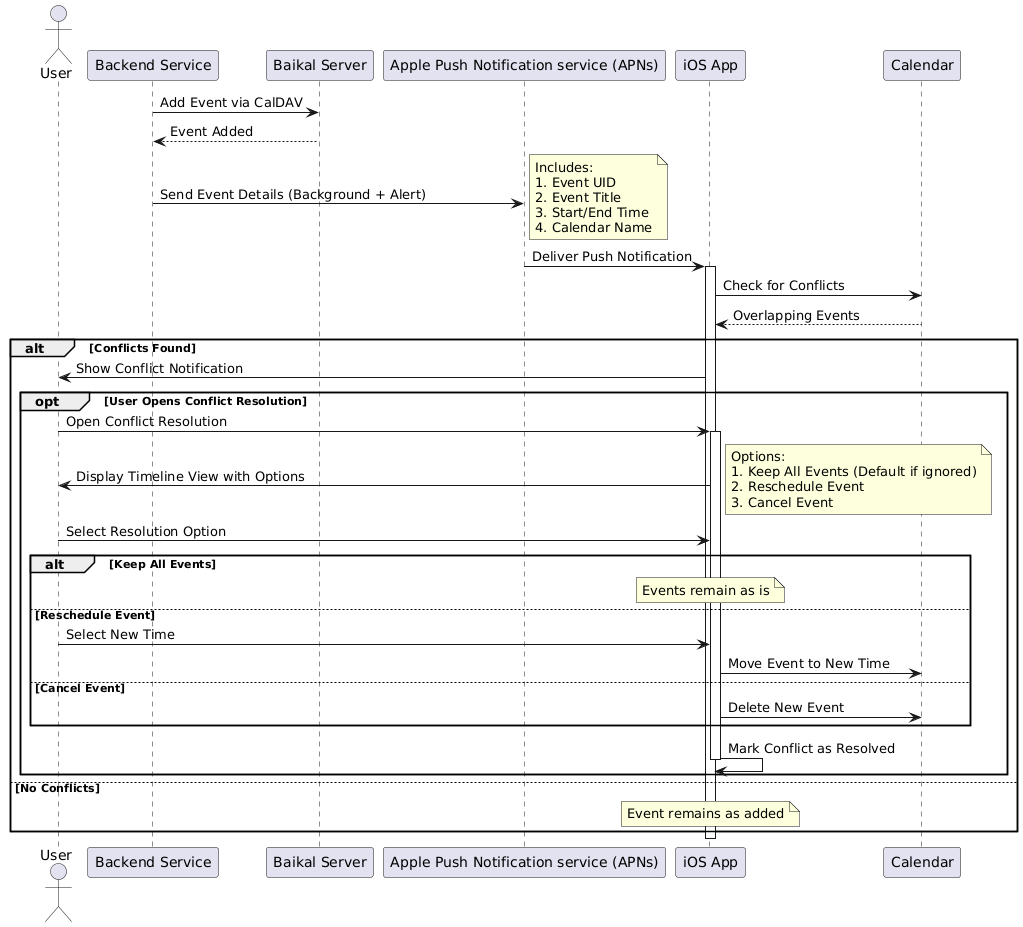
\includegraphics[width=\textwidth]{images/docs/diagrams/sequence-diagrams/all-sequence-diagrams/Suggest Conflict Resolutions.png}
  \caption{Suggest Conflict Resolutions Sequence Diagram}
  \label{fig:seq/suggest-conflict-resolutions}
\end{figure}

The sequence diagram in Figure~\ref{fig:seq/suggest-conflict-resolutions} illustrates the conflict detection and resolution workflow in Jadwal. When events are added to the calendar (either manually or through WhatsApp extraction), the System initiates a conflict check in the Database. This check specifically looks for temporal overlaps between events and identifies potential alternative time slots.

If conflicts are detected, the System follows a structured resolution process:
\begin{enumerate}
  \item Retrieves resolution options from the Database, which include:
        \begin{itemize}
          \item Moving the overlapping event to an alternative time slot
          \item Keeping both events with an explicit conflict warning
        \end{itemize}
  \item Obtains the device IDs associated with the customer who owns the conflicting events
  \item Utilizes Apple Push Notification service (APNs) to notify users about the conflict and present them with resolution options
\end{enumerate}

If no conflicts are detected, the System continues without any additional actions. This approach ensures users are promptly informed of scheduling conflicts while maintaining the flexibility to either reschedule events or knowingly maintain overlapping appointments. The workflow aligns with Jadwal's goal of providing straightforward conflict management while respecting user preferences in calendar organization.

This process specifically implements the use case requirements, focusing on practical conflict resolution through user notification and simple resolution options, rather than attempting automated resolution or complex prioritization schemes.